\documentclass[UTF8]{ctexart}
\usepackage{algpseudocode}
\usepackage{algorithm}
\usepackage{amsmath}
\usepackage{subcaption}
\usepackage{graphicx}
\usepackage[top=4em,bottom=4em]{geometry}
\usepackage{lmodern}
\usepackage{listings}
\usepackage{xcolor}

\ctexset{ section = { format={\Large \bfseries } } }

\pagestyle{empty}

\begin{document}

\section*{Task 1: Parallel Coordinates Visualization}

首先统计每种数据的最大最小值作为坐标轴的范围,出于美观考虑在上下各留一定比例的空白,并将最大最小值分别向上和向下取整,方便在图中标注。对于每条坐标轴,模仿 Tutorial 中的参考效果用四条线组合而成。交互的设计是,当鼠标位于某个坐标轴附近的区域时,将该坐标轴高亮,并且每个样本对应的折线的颜色由该样本在该坐标上的位置决定,用两种颜色插值得到。这样可以方便用户观察不相邻维度的相关性。实现效果如下:

\begin{figure}[htbp]
    \centering
    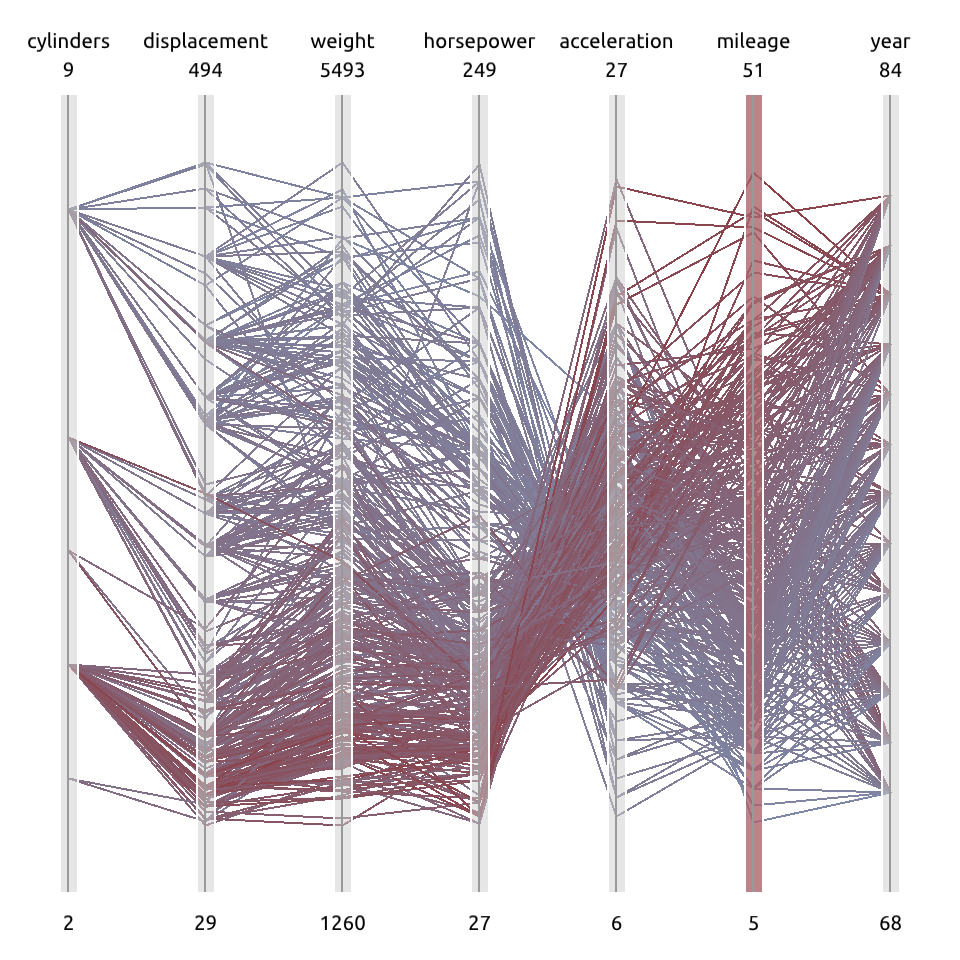
\includegraphics[width=0.8\textwidth]{images/vis.png}
    \caption*{Parallel Coordinates Visualization}
\end{figure}

\end{document}